\documentclass[12pt, twoside]{article}
\usepackage[letterpaper, margin=1in, headsep=0.5in]{geometry}
\usepackage[english]{babel}
\usepackage[utf8]{inputenc}
\usepackage{amsmath}
\usepackage{amsfonts}
\usepackage{amssymb}
\usepackage{tikz}
%\usetikzlibrary{quotes, angles}

\usepackage{graphicx}
\usepackage{enumitem}
\usepackage{multicol}

\usepackage{fancyhdr}
\pagestyle{fancy}
\fancyhf{}
\renewcommand{\headrulewidth}{0pt} % disable the underline of the header

\fancyhead[RE]{\thepage}
\fancyhead[RO]{\thepage \\ Name: \hspace{3cm}}
\fancyhead[L]{BECA / Dr. Huson / 10.3 Geometry\\* 14 January 2019}

\begin{document}
\subsubsection*{Do Now}
  \begin{enumerate}

  \subsubsection*{Quadratic Formula}
      \item Solve $x^2 - 6x - 27 = 0$ by factoring. Then check with the quadratic formula. \vspace{3cm}
      \item Solve $x^2 - 11x  + 13 = 0$. \vspace{3cm}

  \subsubsection*{Fractional Algebra}
      \item $3 + \dfrac{9}{2}(3x - 5) = 21$ \vspace{3cm}
      \item $8 + \dfrac{5}{x}(-7x - 10) = 23$ \vspace{3cm}

  \newpage

  \subsubsection*{Graphing Inequalities}

    \item Solve for $y$, then graph the two inequalities.
        \begin{multicols}{2}
          $2y + 6 < x$ \\
          $y + 3x \geq 8$
        \end{multicols}
        \vspace{2.5cm}

        \begin{center} %4 quadrant regents grid w T-Chart
        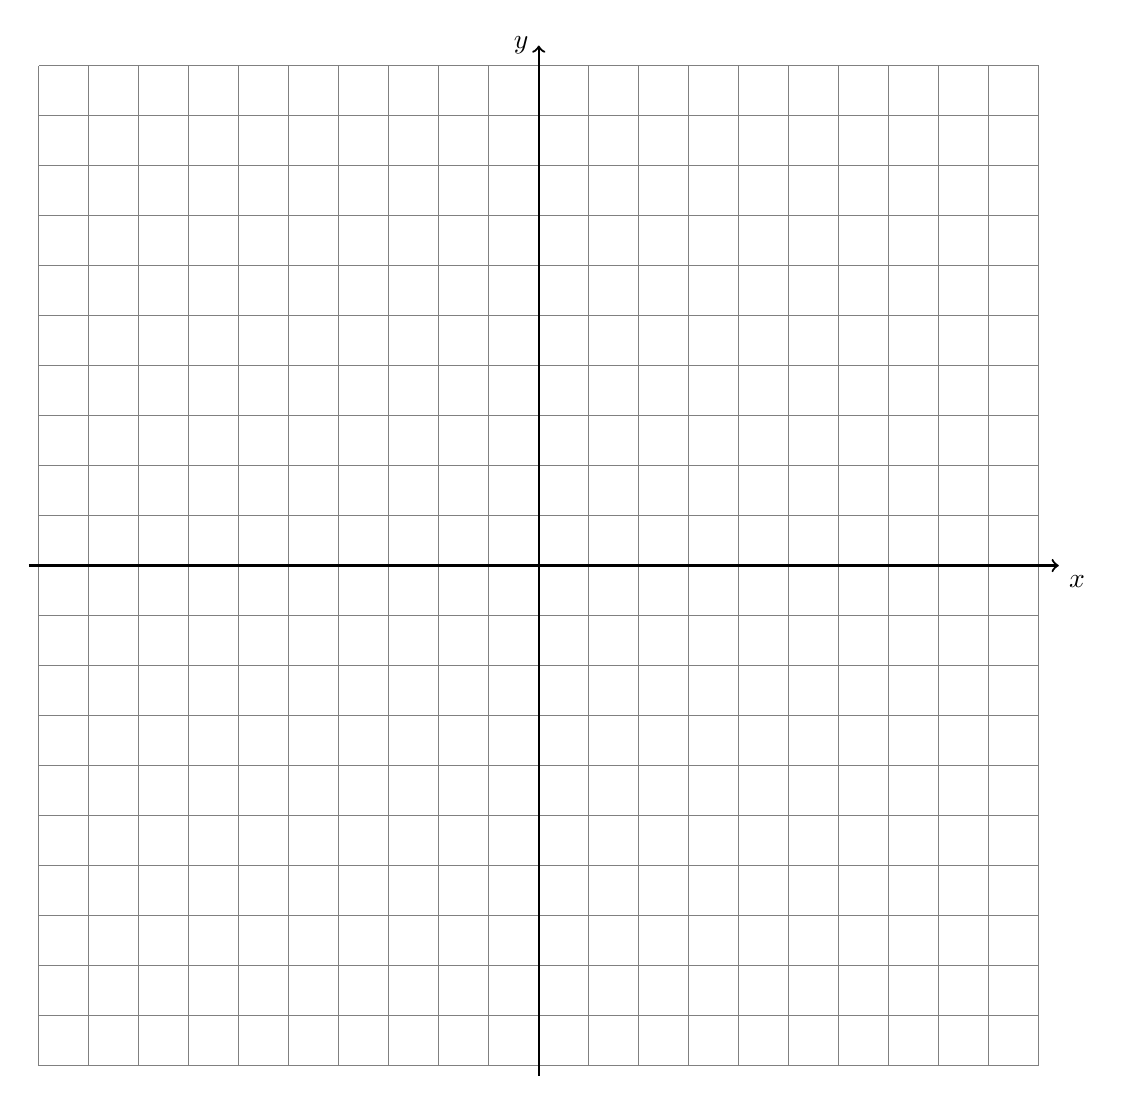
\begin{tikzpicture}[scale=.635]
          \draw [help lines] (-10,-10) grid (10,10);
          \draw [thick, ->] (-10.2,0) -- (10.4,0) node [below right] {$x$};
          \draw [thick, ->] (0,-10.2)--(0,10.4) node [left] {$y$};
        \end{tikzpicture}
        \end{center}

      Mark the solution set with a capital ``S". Are the following points solutions?
      \begin{enumerate}
          \item (2, -2) \vspace{2cm}
          \item (3, -5) \vspace{2cm}
          \item (-1, 7) \vspace{2cm}
      \end{enumerate}

\end{document}
